Today we'll begin our discussion of renormalization and why infinities might not be so scary after all (cf. Skinner \textsection 5.1). Let us consider $\phi^4$ theory:
\begin{equation}
    S[\phi]=\int d^4x \bkt{
        \frac{1}{2} \p_\mu \phi \p^\mu \phi+\frac{1}{2} m^2 \phi^2 +\frac{\lambda}{4!}\phi^4
    }.
\end{equation}
In momentum space, the full propagator $\tilde{\gv \Delta}(p^2)$ takes the form
\begin{equation}
    \tilde{\gv \Delta}(p^2)=\int d^4x\, e^{-ip\cdot x}\avg{\phi(x) \phi(0)}_{\text{connected}}.
\end{equation}
That is, our full propagator is the amplitude to go from one point to another via any connected diagram. There's of course the tree-level way to do it, corresponding to $\Delta = \frac{1}{p^2+m^2}$. But once we introduce interactions, there will be infinitely many diagrams that contribute to this amplitude. However, the idea of 1PI diagrams will allow us to organize this infinite sum in a sensible way.

Schematically, we can represent the propagator as the following sum of diagrams:
\begin{center}
    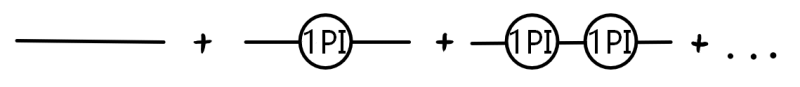
\includegraphics[width=0.75\textwidth]{2019/02/20190209_1piexpansion.png}
\end{center}
or equivalently the following geometric series:
\begin{align*}
    \tilde{\gv \Delta}(p^2) &= 
        \frac{1}{p^2+m^2}+\frac{1}{p^2+m^2} \Pi(p^2) \frac{1}{p^2+m^2} + \frac{1}{p^2+m^2} \Pi(p^2) \frac{1}{p^2+m^2} \Pi(p^2) \frac{1}{p^2+m^2}+\ldots \\
        &=\frac{1}{p^2+m^2-\Pi(p^2)}
\end{align*}
where $\Pi(p^2)$ is called the self-energy. 

Note that $\Pi$ contributes to the quantum effective action $\Gamma$. As can be seen from the form of $\tilde{\gv \Delta}(p^2)$, it has the effect of shifting the parameter $m$, which we previously called the mass-- what this sum tells us is that the ``mass'' $m$ from the Lagrangian is not the same effective mass we would actually measure in the full propagator. It was naive to think we could propagate from one point to another with tree-level diagrams only-- we must account for quantum corrections along the way.

Perturbatively, we get contributions from diagrams like the following:
\begin{center}
    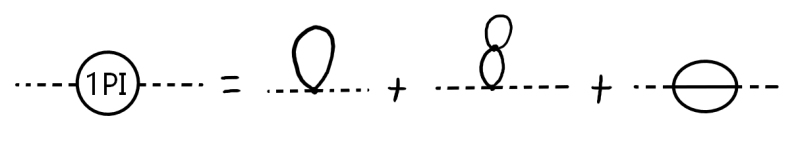
\includegraphics[width=0.75\textwidth]{2019/02/20190209_1pidiagrams.png}
\end{center}
That is, $\Pi$ represents the sum of contributions from all 1PI diagrams with two external legs. Note that the dashed lines are omitted from the computation of the 1PI factor $\Pi(p^2)$ since they are external propagators and already accounted for in our expansion.

One of the simplest propagator corrections we can draw in $\phi^4$ theory is the one-loop diagram, and it corresponds to the amplitude
\begin{equation}
    -\frac{\lambda}{2}\int \frac{d^4k}{(2\pi)^4} \frac{1}{k^2+m^2}.
\end{equation}
This is divergent, since the integral goes as $d^4k/k^2$. To see this explicitly, let us introduce an ultraviolet (UV) cutoff $\Lambda$ so that we integrate over only momenta with $|k|<\Lambda$. Since the integral depends only on $k^2$, we can change to spherical coordinates and integrate:
\begin{equation}
    -\frac{\lambda S_4}{2(2\pi)^4} \int_0^\Lambda \frac{k^3 dk}{k^2+m^2}=-\frac{\lambda S_4 m^2}{4(2\pi)^4} \int_0^{\Lambda^2/m^2}\frac{u du}{1+u} = -\frac{\lambda}{32\pi^2} \bkt{\Lambda^2 - m^2 \log \paren{1+\frac{\Lambda^2}{m^2}}},
\end{equation}
where $d^dk= S_d |k|^{d-1} d|k|$ with $S_d=\frac{2\pi^{d/2}}{\Gamma(d/2)}$ and we've made the substitution $u=k^2/m^2$ to perform the integral.%
    \footnote{Quick note: that gamma function in the volume of the $d-1$-sphere will be nice in even dimension, and somewhat less nice in odd dimension. Here, we have $d=4$, so that $\Gamma(d/2)=\Gamma(2)=1!=1$, and the numerator is just $2\pi^2$. In odd dimension, we evaluate the gamma function at a half-integer, and its value is given by a weird double factorial: $\Gamma\paren{n+\frac{1}{2}}=\frac{(2n-1)!!}{2^n} \sqrt{\pi},$ where $n!!=(n)(n-2)(n-4)\ldots 3\cdot 1$ for odd $n$.
    }
After performing the integral, we arrive at an amplitude that indeed diverges as $\Lambda\to\infty$.

\subsection*{Counterterms} 
Obviously, physical propagators are not infinite, yet our Feynman rules seem to have given us a divergent amplitude for a simple one-loop correction. How can we make our theory sensible again? Instead of working with the original Lagrangian (sometimes called the ``bare Lagrangian''), suppose we allow the coupling to depend on $\Lambda$ by adding ``counterterms'' to the action. That is, we modify the action to include terms which depend explicitly on the cutoff $\Lambda$:
\begin{equation}
    S[\phi] \to S[\phi]+(\hbar)S^{CT}[\phi,\Lambda].
\end{equation}
For instance, we might define a set of counterterms as
\begin{equation}
    S^{CT}[\phi,\Lambda]=\int d^4x \bkt{
        \frac{\delta Z(\Lambda)}{2} \p_\mu \phi \p^\mu \phi +\frac{1}{2} \delta m^2(\Lambda) \phi^2 +\frac{\delta \lambda(\Lambda)}{4!} \phi^4
    }.
\end{equation}
These counterterms correspond to some new vertices and thus new contributions to $\Pi(p^2)$. The $\delta Z$ coupling will contribute to a new (momentum-dependent) two-point vertex, as will the $\delta m^2$ coupling:
\begin{center}
    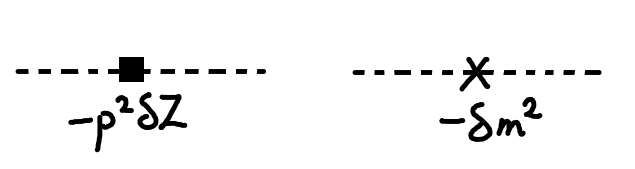
\includegraphics[width=0.5\textwidth]{2019/02/20190209_1loopcorrections.png}
\end{center}

At 1 loop, the sum of 1PI diagrams with two external legs becomes
\begin{equation}\label{phi4selfenergy}
    \Pi^{\text{1-loop}}(p^2)=-p^2 \delta Z -\delta m^2 -\frac{\lambda}{32\pi^2}\bkt{\Lambda^2-m^2\log \paren{1+\frac{\Lambda^2}{m^2}}}.
\end{equation}
At two loops, the three counterterm diagrams
\begin{center}
    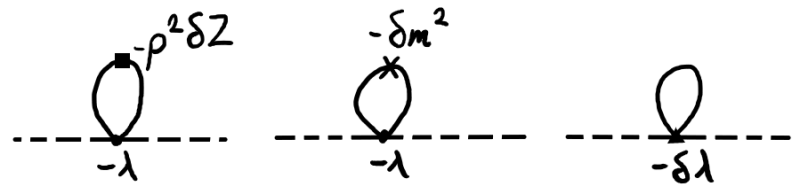
\includegraphics[width=0.75\textwidth]{2019/02/20190209_2loopcorrections.png}
\end{center}
must also be included.%
    \footnote{
        Note that all these diagrams visually look like they only have one loop. What's going on? Basically, there's a factor of $\hbar$ that suppresses all of the counterterm couplings. What we're really doing is expanding in powers of $\hbar$ and/or $\lambda$, since it was the four-point $\lambda$ coupling that gave rise to loops even before we introduced our counterterms. Thus the first two diagrams pick up a factor of $\lambda$ from the original action and an $\hbar$ from the counterterm couplings $\delta Z, \delta m^2$. The third diagram corresponds to the $\delta \lambda$ coupling, which is part of the counterterms and so has a factor of $\hbar$ but is also a $\lambda$ correction itself, and so is treated at two loop order.
        
        Put more simply (as Skinner says), each counterterm vertex counts as a loop.
    }
Now we can tune the parameters $\delta Z, \delta m^2, \delta \lambda$ in our counterterms to cancel the divergences to some loop order. In other words, we \term{renormalize} $\phi,m^2,\lambda$.

\subsection*{On-shell renormalization scheme}
The need to ``regulate'' the theory by cancelling divergences does not uniquely determine the counterterms, so we impose additional renormalization conditions, which we call a \term{scheme}. It will turn out that physical observables do not depend on our choice of scheme.

The on-shell scheme is as follows. We fix $\delta Z, \delta m^2, \delta \lambda$ by requiring that
\begin{enumerate}
    \item[1.] $\tilde {\gv \Delta}(p^2)$ has a simple pole at some experimentally observable mass, i.e. for $p^2=-m^2_{\text{phys}}$, and
    \item[2.] The residue of this pole is equal to $1$.
\end{enumerate}
Therefore since
\begin{equation}
    \tilde {\gv \Delta}(p^2)=\frac{1}{p^2+m^2-\Pi(p^2)},
\end{equation}
our first condition says that
\begin{equation}
    \Pi(p^2=-m^2_{\text{phys}})=m^2-m^2_{\text{phys}}.
\end{equation}
We can additionally set $m^2-m^2_{\text{phys}}=0$ if we want the mass in $\cL$ to equal $m_{\text{phys}}$ at this order of counterterm.
Imposing the second condition then tells us that
\begin{equation}
    \P{\Pi}{p^2}|_{p^2=-m_{\text{phys}}^2}=0,
\end{equation}
by L'H\^opital's rule.%
    \footnote{
        This is a little quick. Recall that for a function $f(z)$ with a simple pole at $z_0$, the residue is the value $\lim_{z\to z_0} f(z)(z-z_0).$ Here, we want $\frac{1}{p^2+m^2+\Pi(p^2)}$ to have unit residue at the pole $p^2=-m_\text{phys}^2$. So the residue is
        \begin{equation*}
            \lim_{p^2\to -m_\text{phys}^2} \frac{p^2+m_\text{phys}^2}{p^2+m^2+\Pi(p^2)} = \lim_{p^2\to -m_\text{phys}^2}\frac{1}{1+\P{\Pi}{p^2}}= \frac{1}{1+\left.\P{\Pi}{p^2}\right\rvert_{p^2=-m_\text{phys}^2}}.
        \end{equation*}
        Setting this expression equal to $1$ gives us precisely the desired condition,
        \begin{equation*}
            \P{\Pi}{p^2}|_{p^2=-m_{\text{phys}}^2}=0.
        \end{equation*}
    }
If we now compare to the expression for the self-energy at one loop, Eqn. \ref{phi4selfenergy}, we see that the second condition gives
\begin{equation}
    \P{\Pi}{p^2}|_{p^2=-m_{\text{phys}}^2}=0 \implies \delta Z=0,
\end{equation}
and the first condition gives
\begin{equation}
    \Pi(-m^2_{\text{phys}})=m^2-m^2_{\text{phys}} \implies \delta m^2= -\frac{\lambda}{32\pi^2} \bkt{\Lambda^2-m^2\log \paren{1+\frac{\Lambda^2}{m^2}}}.
\end{equation}

Note that $\delta Z$ turned out to be zero and we were able to set $\Pi(p^2)=0 \,\forall p^2$ because the one-loop correction to the propagator in $\phi^4$ theory does not depend on the external momentum $p^2$. If we instead tried to construct the counterterms to account for the two-loop diagram (order $\lambda^2$), we would get $\delta Z\neq 0$ since the integral depends on $p$, i.e. the integral corresponding to the diagram
\begin{center}
    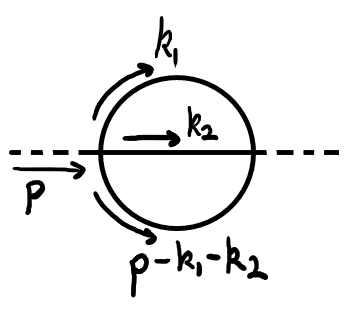
\includegraphics[width=0.3\textwidth]{2019/02/20190209_twolooprenorm.png}
\end{center}
It's worth noting that the counterterm $\delta Z$ is related to the concept of ``wavefunction renormalization.'' That is, it corresponds to a correction to the kinetic term of the original Lagrangian, $\frac{1}{2}\p_\mu \phi \p^\mu\phi$. The kinetic term is special in renormalization because it comes with a canonical normalization of $1/2$, unlike the other couplings which have arbitrary starting values. When we perform the procedure of renormalization group flow to study how couplings change after scaling, it is the kinetic term which will lead to the so-called ``anomalous dimension'' of the field. We'll discuss this more in future lectures.

In general, UV divergences are not too hard to spot-- we saw that
\begin{equation}
    \int^\Lambda \frac{d^4k}{(2\pi)^4} \frac{1}{k^2 +m^2} \sim \Lambda^2,
\end{equation}
and generically
\begin{equation}
    \int^\Lambda \frac{d^nk}{k^m}\sim \begin{cases}
        \Lambda^{n-m}, & n\neq m\\
        \log \Lambda, & n = m.
    \end{cases}
\end{equation}

\subsection*{Non-lectured aside: renormalization}

It's worth taking a minute to think about what we're really doing here in renormalizing our theory. To recap, we wrote down a bunch of Lagrangians and actions last term. We derived their Feynman rules, and used the Feynman rules to make some computations of matrix elements, scattering amplitudes, and other physically important quantities.

But there was a trap hidden in our attempt to write down quantum field theories. The Feynman rules tell us that strictly, we should include loop diagrams in our calculations, though the corrections from those diagrams are in principle suppressed by additional factors of the coupling constant. A priori, this sounds like it's not too bad. But once we start writing down loop diagrams and integrating over loop momenta, what we discover is that these corrections we hoped were small are in fact infinite. The integrals over momentum generically diverge, and no factors of the coupling constant can suppress an infinity.

So what do we do? A pragmatic first step to remedying this problem is to say that our theory simply isn't valid to arbitrarily large momentum. As physicists, we know that at very high energies, different forces may unify and perhaps quantum gravitational effects are significant, so it's simply a question of admitting our ignorance and treating our theory as an effective theory at low energies.

But now that we have this cutoff, we would still like to make predictions with our theory that don't depend on our choice of cutoff. Renormalization allows us to do this. It tells us that our first attempt at writing down the actions of quantum field theories was wrong, since it had divergences baked into it from the very beginning. Instead, what we should really be working with is a renormalized effective theory, i.e. we add in counterterms to modify the original couplings to precisely cancel the divergences at some desired order.

This is a very practical thing to do, because once we make some measurements of actual scattering amplitudes, we can fix the values of the couplings in our effective theories and make predictions using for instance the physical mass of a particle (i.e. the effective mass), rather than some mysterious constant $m$ which we can never actually measure. What would have been an honest mass in classical field theory becomes impossible to measure once we add in quantum corrections-- the physically relevant thing is then $m_{\text{phys}}$ (though we can sometimes set $m^2=m_{\text{phys}}^2$ by a choice of scheme), and the same is true of other coupling constants.